\documentclass[11pt]{article}
\usepackage{neurips_2024}
\usepackage{graphicx}
\usepackage{booktabs}
\usepackage{amsmath}
\usepackage{hyperref}
\usepackage{caption}
\usepackage{subcaption}
\usepackage{enumitem}
\setlist{nosep}

\title{Multi-source Asset Generation and Real-scene Fusion with 3DGS and AIGC}
\author{Deep Learning and Spatial Intelligence Final Project, Task 1}
\date{}

\begin{document}
\maketitle

\begin{abstract}
This project builds an end-to-end 3D visual pipeline for multi-source asset generation and real-scene fusion. Object A is reconstructed from real multi-view images with COLMAP and 3D Gaussian Splatting (3DGS). Object B is generated from text using threestudio with SDS guidance, and Object C is generated from a single foreground image using Zero123. The background is the garden scene from Mip-NeRF 360, reconstructed with 3DGS. Finally, the three assets are inserted into the same garden world coordinate system and rendered as a multi-view orbit video. The final renderer uses a hybrid representation: garden and Object A are rendered as explicit Gaussians, while Object B and C are exported as textured meshes and composited with the same camera trajectory and depth ordering.
\end{abstract}

\section{Project Links}
\textbf{GitHub:} \href{https://github.com/jiangjingshuang2-stack/Deep-Learning-Final}{github.com/jiangjingshuang2-stack/Deep-Learning-Final}.\\
\textbf{Model weights:} \href{https://drive.google.com/drive/folders/154-pIcfsTkYXpTeUgTcfOjBJ5Sep0xIy?dmr=1&ec=wgc-drive-%5Bmodule%5D-goto}{Google Drive model weights folder}.\\
\textbf{Main output video:} \texttt{videos/final\_ABC\_garden\_world\_static\_v2.mp4}.

\section{Background}
The assignment requires a complete 3D pipeline that combines real-world reconstruction, AIGC-based 3D asset generation, and real-scene rendering. 3DGS represents a scene as colored, anisotropic 3D Gaussians and enables efficient high-quality rendering. In contrast, AIGC models often produce implicit fields or textured meshes. Therefore, the main challenge of the final stage is to align coordinate systems, scales, representations, and visibility.

\section{Data and Assets}
\textbf{Object A} is reconstructed from real multi-view images. The foreground images are rotated clockwise by 90 degrees before COLMAP pose estimation. With a relaxed full-frame pinhole setting, 71 valid camera poses are recovered and used for 3DGS training.

\textbf{Object B} is generated using threestudio with the following prompt:
\begin{quote}
\texttt{a small blue ceramic dragon statue, detailed scales, glossy surface, studio lighting}
\end{quote}

\textbf{Object C} is generated from a single background-removed sunscreen image using Zero123.

\textbf{Background} is the garden scene from the Mip-NeRF 360 dataset, trained with 3DGS for 30000 iterations.

\section{Method}
\subsection{Multi-view Reconstruction for Object A}
COLMAP first estimates camera intrinsics, extrinsics, and a sparse point cloud. 3DGS then optimizes Gaussian positions, covariance, opacity, and spherical-harmonic colors. The reconstruction loss combines an L1 color term and a D-SSIM term:
\begin{equation}
\mathcal{L}=(1-\lambda)\mathcal{L}_{1}+\lambda \mathcal{L}_{D-SSIM}.
\end{equation}

\subsection{Text-to-3D Generation for Object B}
Object B is optimized with SDS guidance. Random views of the current 3D representation are rendered, and a pretrained 2D diffusion model provides gradient guidance. This path requires only a prompt, but its geometry is weaker than multi-view reconstruction and depends heavily on diffusion priors.

\subsection{Single-image-to-3D Generation for Object C}
Object C uses Zero123 to infer novel-view consistency from one foreground image. Compared with text-to-3D generation, the input image provides stronger appearance constraints, especially for the front view, while invisible regions still require generative completion.

\subsection{Garden Background Reconstruction}
The garden scene is trained with 3DGS from the Mip-NeRF 360 multi-view images. It provides the real-scene coordinate system and the camera path for final rendering.

\subsection{Representation Unification and Fusion}
The final pipeline uses a hybrid representation. Garden and Object A are both explicit 3D Gaussians, so Object A is filtered, normalized, transformed, and inserted into the garden world coordinate system. Object B and C are exported as textured meshes from threestudio, normalized, converted from the local generated coordinate system to the garden camera/world convention, and fixed in the same world space. Rendering first produces garden + A frames using the official 3DGS renderer. B and C are then rasterized and depth-composited with the same camera trajectory. This makes the assets world-static relative to the background during the orbit.

\section{Experimental Setup}
\begin{table}[H]
\centering
\caption{Main experimental settings.}
\begin{tabular}{lllll}
\toprule
Asset & Method & Steps & Input & Output \\
\midrule
A & COLMAP + 3DGS & 7000 & 71 valid multi-view images & Gaussian PLY \\
B & DreamFusion / SDS & 5000 & Text prompt & Textured mesh \\
C & Zero123 & 600 & One foreground image & Textured mesh \\
garden & 3DGS & 30000 & Mip-NeRF 360 garden & Gaussian PLY \\
\bottomrule
\end{tabular}
\end{table}

\begin{table}[H]
\centering
\caption{Hyperparameters and logs.}
\resizebox{0.96\linewidth}{!}{%
\begin{tabular}{llll}
\toprule
Experiment & Optimizer / Loss & Key setting & Log \\
\midrule
A 3DGS & Adam, L1 + D-SSIM & iter=7000, GPU=2 & \texttt{objectA\_3dgs\_train\_7000.log} \\
B SDS & Adam, SDS loss & steps=5000, GPU=3 & W\&B run \texttt{7txhb0k5} \\
C Zero123 & Adam, Zero123 guidance & steps=600, GPU=0 & W\&B run \texttt{4azkmnu1} \\
garden 3DGS & Adam, L1 + D-SSIM & iter=30000, GPU=2 & \texttt{garden\_3dgs\_train\_30k...log} \\
\bottomrule
\end{tabular}
}
\end{table}

\begin{table}[H]
\centering
\caption{Detailed training and evaluation settings.}
\resizebox{0.96\linewidth}{!}{%
\begin{tabular}{llllll}
\toprule
Experiment & Network Architecture & Batch Size & Learning Rate & Epochs/Steps & Metrics \\
\midrule
A & 3D Gaussian, SH color & 1 view/iter & default 3DGS schedule & 7000 iter & L1, PSNR \\
B & threestudio NeRF/mesh export & 1 view/iter & default Adam & 5000 steps & SDS loss, render check \\
C & Zero123-guided 3D field & 1 view/iter & default Adam & 600 steps & guidance loss, render check \\
garden & 3D Gaussian, SH color & 1 view/iter & default 3DGS schedule & 30000 iter & L1, PSNR \\
\bottomrule
\end{tabular}
}
\end{table}

\begin{table}[H]
\centering
\caption{Key evaluation metrics.}
\begin{tabular}{llll}
\toprule
Experiment & Split & L1 $\downarrow$ & PSNR $\uparrow$ \\
\midrule
A 3DGS & test @ 7000 & 0.00943 & 25.97 \\
A 3DGS & train @ 7000 & 0.00478 & 31.81 \\
garden 3DGS & train @ 30000 & 0.02038 & 30.04 \\
C Zero123 & train @ 600 & 2.30 & -- \\
\bottomrule
\end{tabular}
\end{table}

\section{Results}
\begin{figure}[H]
\centering
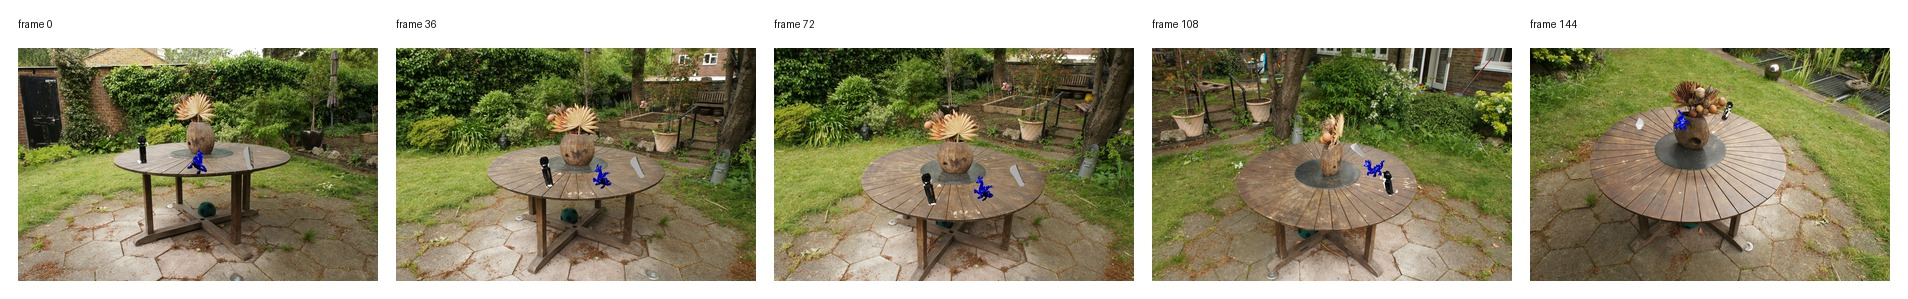
\includegraphics[width=\linewidth]{figures/fusion_world_static_v2_contact.jpg}
\caption{Representative frames from the final v2 fusion video. The assets and the garden background are fixed in the same world coordinate system.}
\end{figure}

\begin{figure}[H]
\centering
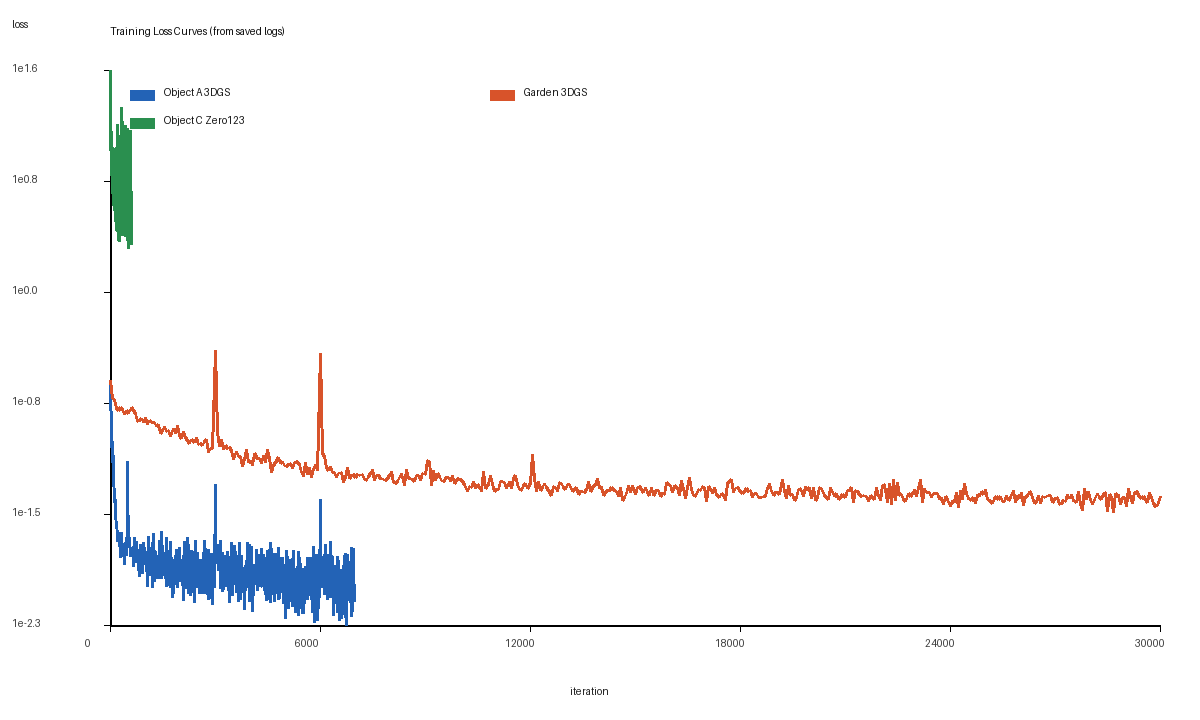
\includegraphics[width=0.85\linewidth]{figures/loss_curves_all.png}
\caption{Training curves parsed from saved logs. The console log for Object B does not contain scalar loss values; the complete scalar records are available in the W\&B run.}
\end{figure}

\begin{figure}[H]
\centering
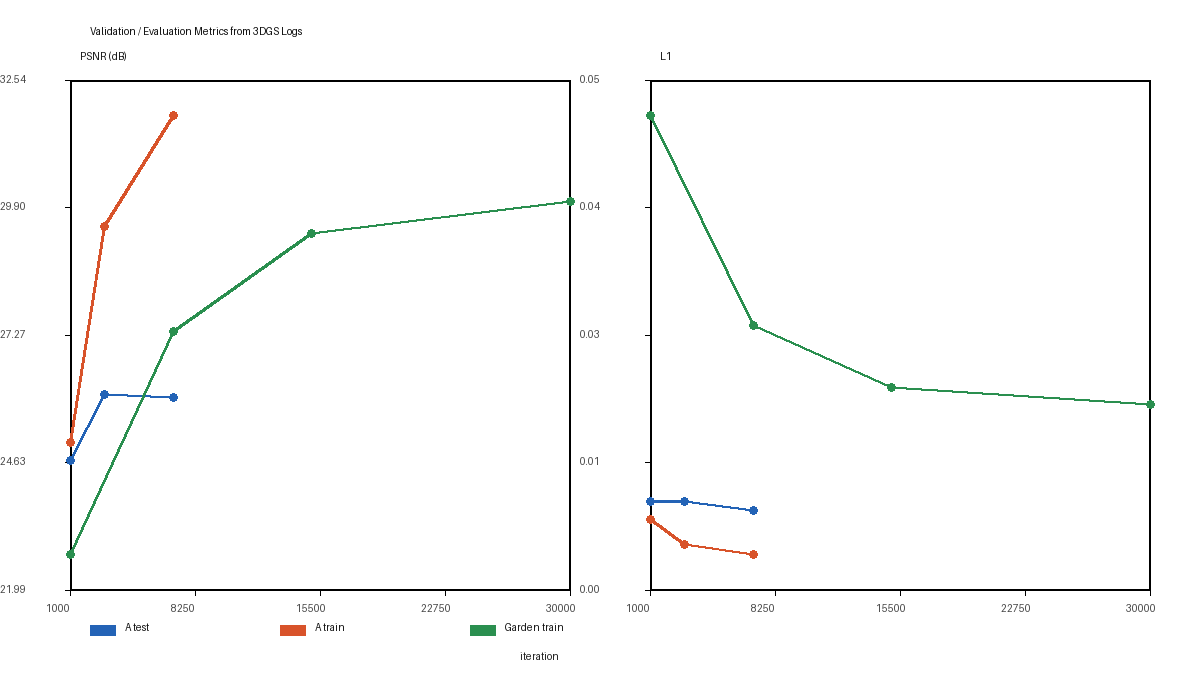
\includegraphics[width=0.85\linewidth]{figures/validation_metrics_3dgs.png}
\caption{Validation/evaluation curves. Object A includes train/test L1 and PSNR. The garden log records train L1 and PSNR. B/C are mainly monitored through W\&B guidance losses and exported render checks.}
\end{figure}

\begin{figure}[H]
\centering
\begin{subfigure}{0.48\linewidth}
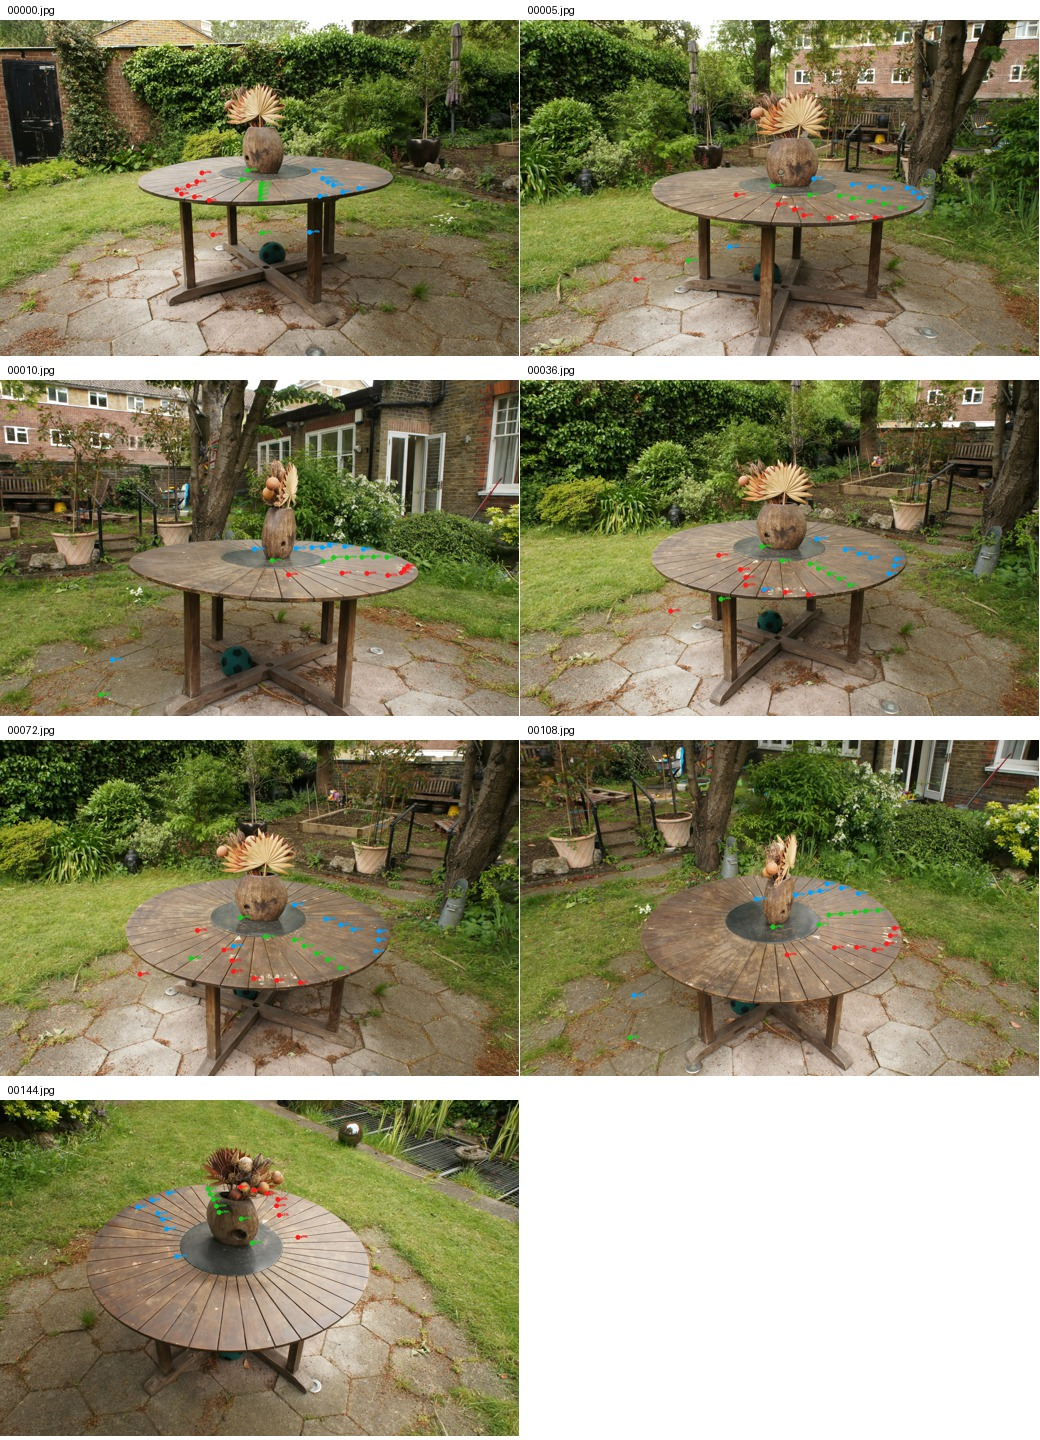
\includegraphics[width=\linewidth]{figures/table_candidates.jpg}
\caption{Candidate table points}
\end{subfigure}
\begin{subfigure}{0.48\linewidth}
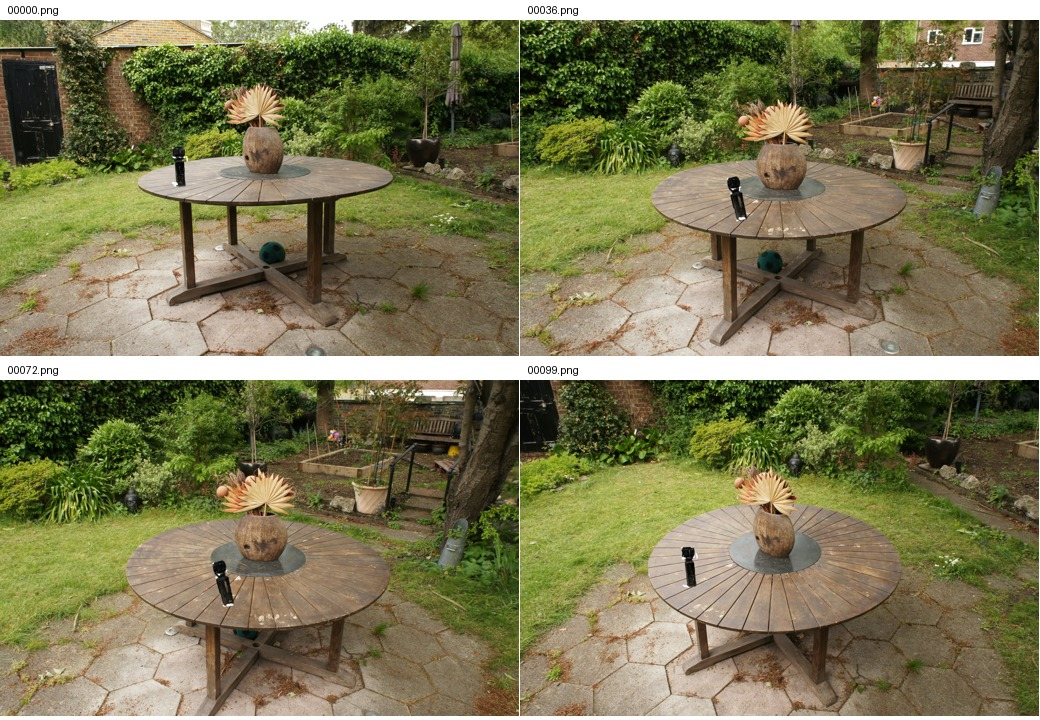
\includegraphics[width=\linewidth]{figures/a_v2_position_check.jpg}
\caption{Object A after upward adjustment}
\end{subfigure}
\caption{Fusion position debugging. In v2, Object A is slightly lifted to reduce table occlusion.}
\end{figure}

\section{Comparison}
\begin{table}[H]
\centering
\caption{Comparison of the three asset generation paths.}
\resizebox{0.96\linewidth}{!}{%
\begin{tabular}{llll}
\toprule
Path & Geometry & Texture & Cost and stability \\
\midrule
Multi-view A & Highest, pose-dependent & Real texture, image-quality dependent & Medium cost, stable after COLMAP succeeds \\
Text-to-3D B & Prior-driven, less constrained & Stylized, may lack real details & Prompt-only, but less stable geometry \\
Single-image C & Accurate front, hallucinated back & Strong front-view texture & Lower cost, sensitive to image quality \\
\bottomrule
\end{tabular}
}
\end{table}

The multi-view path provides the most faithful real geometry and appearance. The text-to-3D path is useful for rapid concept asset generation, but the dragon shape is easier to recognize in the standalone render than in the final garden scene because the final camera path is determined by the background. The single-image path preserves the visible appearance well but still relies on generative completion for unobserved regions.

\section{Discussion}
The main difficulty for Object A is robust pose recovery from foreground object images. Relaxed matching and the full-frame pinhole setting increase the number of valid poses to 71. In the final fusion, Object A was initially too low and partly occluded by the table surface; the v2 video lifts it slightly while preserving the world-static relationship.

For Object B, the generated mesh looked clearer in the standalone orbit. In the full garden scene, scale, viewing distance, and occlusion reduce the recognizability of the dragon. The final version therefore focuses on correct world-space fusion instead of screen-space overlay.

\section{Conclusion}
The project completes a full pipeline from real capture and AIGC asset generation to 3DGS scene reconstruction and final fusion rendering. The submission includes standalone videos for A/B/C/garden, the final ABC+garden world-static video, training logs, fusion scripts, and bilingual LaTeX report sources. The experiments show that 3DGS is highly effective for real-scene reconstruction, while AIGC assets require careful coordinate, scale, and visibility alignment before they can be integrated into a real 3D scene.

\end{document}
